\documentclass [aspectratio=169]{beamer}
\beamertemplatenavigationsymbolsempty
\usetheme{Boadilla}
\usepackage{textpos} % package for the positioning
\usepackage[]{graphicx}
\usepackage{graphicx}
\usepackage{float}
\usepackage{hyperref}
\usepackage{caption}
\usepackage{subcaption}
\usepackage{algorithm,algpseudocode}
\usepackage[export]{adjustbox}
\usepackage{tikz}
\usepackage[square,numbers]{natbib}
\usepackage[byname]{smartref}
\usetikzlibrary{positioning}
\usetikzlibrary{arrows, shapes, decorations, automata, backgrounds, fit, petri, calc}

\newcommand*{\logofont}{\fontfamily{phv}\selectfont}

\definecolor{uwopurple}{RGB}{79,38,131} % official purple color for uwo

\title[]{\vspace{60pt} \\
Zen and the art of \bbonu\ searches} % Change the lecture topic right here!
\subtitle{KamLAND-ZEN}
\author[]{J.J. Gómez Cadenas}
\institute[]{Donostia International Physics Center}
\date{\today}

% Math notations
\newtheorem{thm}{Theorem}[section]
\newtheorem{lem}[thm]{Lemma}

\newtheorem{defn}[thm]{Definition}
\newtheorem{eg}[thm]{Example}
\newtheorem{ex}[thm]{Exercise}
\newtheorem{conj}[thm]{Conjecture}
\newtheorem{cor}[thm]{Corollary}
\newtheorem{claim}[thm]{Claim}
\newtheorem{rmk}[thm]{Remark}

\newcommand{\ie}{\emph{i.e.} }
\newcommand{\cf}{\emph{cf.} }
\newcommand{\into}{\hookrightarrow}
\newcommand{\dirac}{\slashed{\partial}}
\newcommand{\bbonu}{\ensuremath{\beta\beta0\nu}}
\newcommand{\bbtnu}{\ensuremath{\beta\beta2\nu}}
\newcommand{\mbb}{\ensuremath{m_{\beta\beta}}}
\newcommand{\qbb}{\ensuremath{Q_{\beta\beta}}}
\newcommand{\mbbsq}{\ensuremath{m_{\beta\beta}^2}}
\newcommand{\tonu}{\ensuremath{(T_{1/2}^{0\nu})^{-1}}}
\newcommand{\gonu}{\ensuremath{G^{0\nu}}}
\newcommand{\monu}{\ensuremath{| M^{0\nu}|^2}}
\newcommand{\XE}{\ensuremath{{}^{136}{\rm Xe}}}
\newcommand{\XES}{\ensuremath{{}^{137}{\rm Xe}}}
\newcommand{\GE}{\ensuremath{{}^{76}{\rm Ge}}}
\newcommand{\TE}{\ensuremath{{}^{130}{\rm Te}}}
\newcommand{\TL}{\ensuremath{{}^{208}{\rm Tl}}}
\newcommand{\BI}{\ensuremath{{}^{214}{\rm Bi}}}
\newcommand{\MO}{\ensuremath{{}^{100}{\rm Mo}}}
\newcommand{\KR}{\ensuremath{{}^{83}{\rm Kr}}}
\newcommand{\nne}{\ensuremath{\bar{N}_e}}
\newcommand{\nng}{\ensuremath{\bar{N}_\gamma}}
\newcommand{\so}{\ensuremath{\rm S_1}}
\newcommand{\st}{\ensuremath{\rm S_2}}
\newcommand{\tz}{\ensuremath{\rm t_0}}
\newcommand{\R}{\mathbb{R}}
\newcommand{\C}{\mathbb{C}}
\newcommand{\Z}{\mathbb{Z}}
\newcommand{\N}{\mathbb{N}}
\newcommand{\Q}{\mathbb{Q}}
\newcommand{\LieT}{\mathfrak{t}}
\newcommand{\T}{\mathbb{T}}
\newcommand{\A}{\mathds{A}}
\newcommand{\E}{\mathbb{E}}
\newcommand{\Prob}{\mathbb{P}}
\newcommand{\Var}{\text{Var}}
\newcommand\equalhat{%
\let\savearraystretch\arraystretch
\renewcommand\arraystretch{0.3}
\begin{array}{c}
\stretchto{
    \scalerel*[\widthof{=}]{\wedge}
    {\rule{1ex}{3ex}}%
}{0.5ex}\\ 
=%
\end{array}
\let\arraystretch\savearraystretch
}

% set color
\setbeamercolor{title in head/foot}{bg=white}
\setbeamercolor{author in head/foot}{bg=white}
\setbeamercolor{date in head/foot}{fg=uwopurple}
\setbeamercolor{date in head/foot}{bg=white}
\setbeamercolor{title}{fg=uwopurple}
\setbeamerfont{title}{series=\bfseries}
\setbeamercolor{frametitle}{fg=uwopurple}
\setbeamerfont{frametitle}{series=\bfseries}
\setbeamercolor{block title}{bg=uwopurple!30,fg=black}
\setbeamercolor{item}{fg=uwopurple}
\setbeamercolor{caption name}{fg=uwopurple!70!}


% set logo at non-title pages
%\logo{
\includegraphics[height=0.9cm]{dipc.png}\vspace*{-.45\paperheight}\hspace*{.50\paperwidth}}

\begin{document}

{
\setbeamertemplate{logo}{}
\begin{frame}
    \titlepage
    \begin{textblock*}{4cm}(0.5cm,-7.3cm)
        
\includegraphics[width=4cm]{dipc.png}
    \end{textblock*}
    \begin{textblock*}{8cm}(5.0cm,-7.0cm)
        \huge \color{uwopurple}{$\Bigr\rvert$ \hspace{0.15cm} \textbf{Lecture 7}} % Change the lecture # right here! 
    \end{textblock*}
\end{frame}
}


\begin{frame}{The KamLAND-ZEN approach to \bbonu}
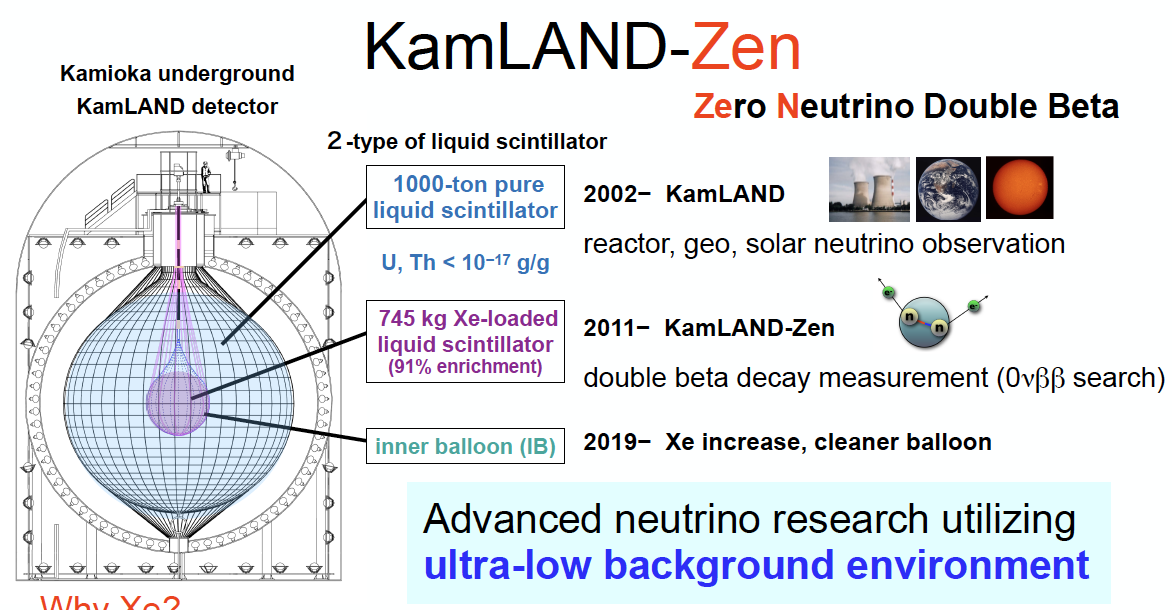
\includegraphics[scale=0.3]{kzen.png}
\end{frame}

\begin{frame}{KamLAND-ZEN phases}
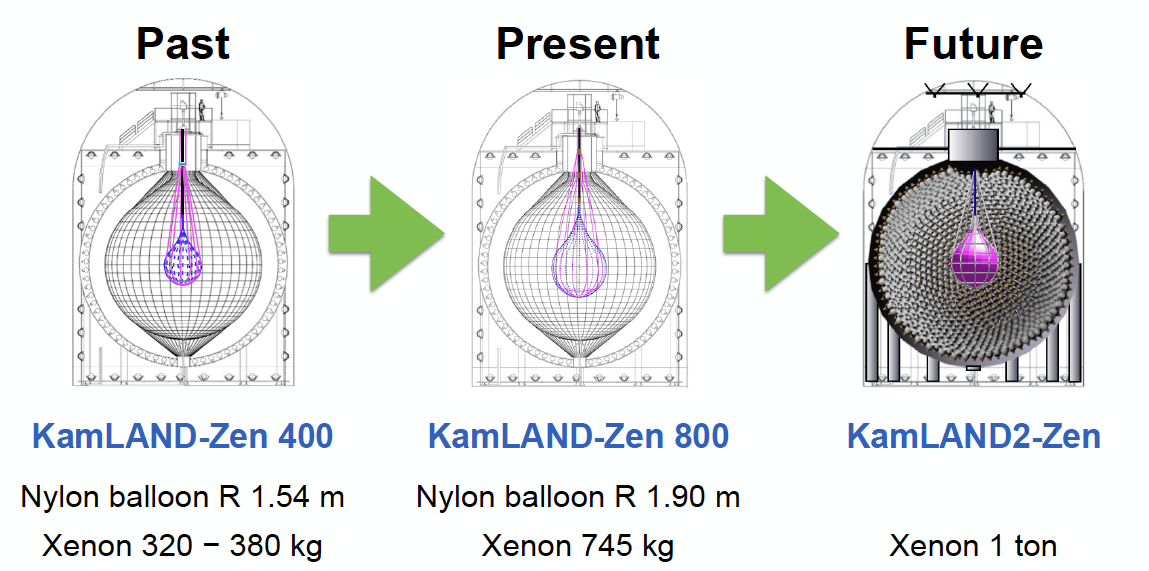
\includegraphics[scale=0.30]{kzenPhases.png}
\end{frame}

\begin{frame}{KamLAND-ZEN baloon}
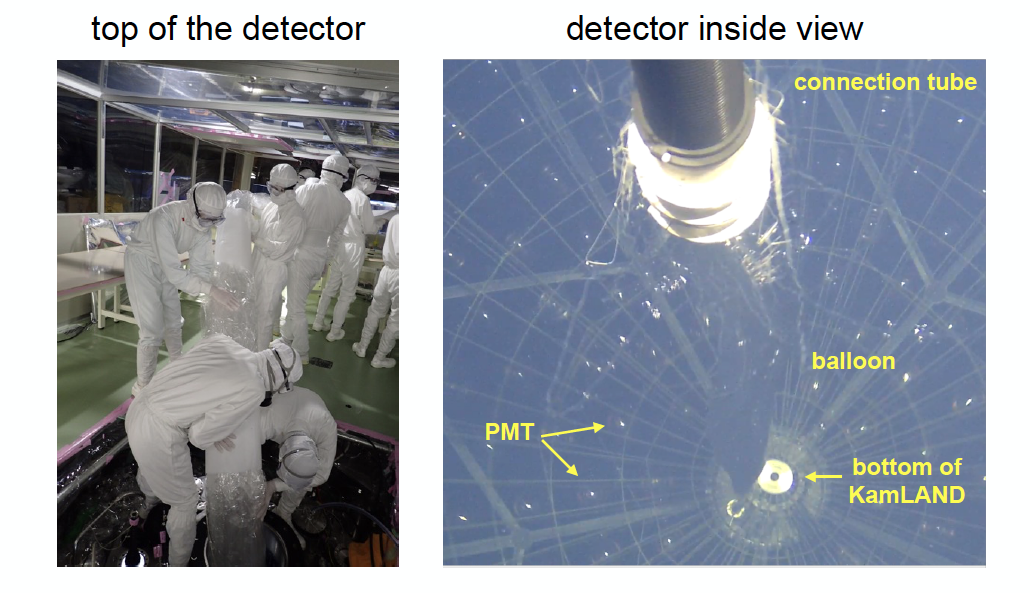
\includegraphics[scale=0.30]{baloon.png}
\end{frame}

\begin{frame}{Background as a function of the radius}
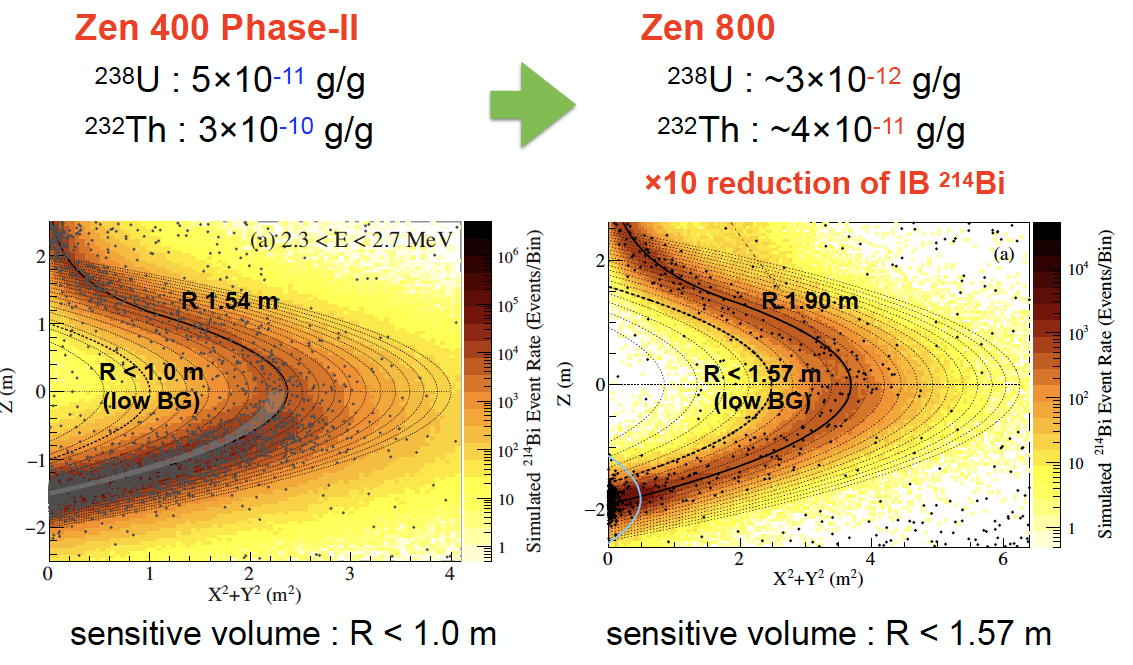
\includegraphics[scale=0.30]{bkgradius.png}
\end{frame}

\begin{frame}{Long-lived spallation products}
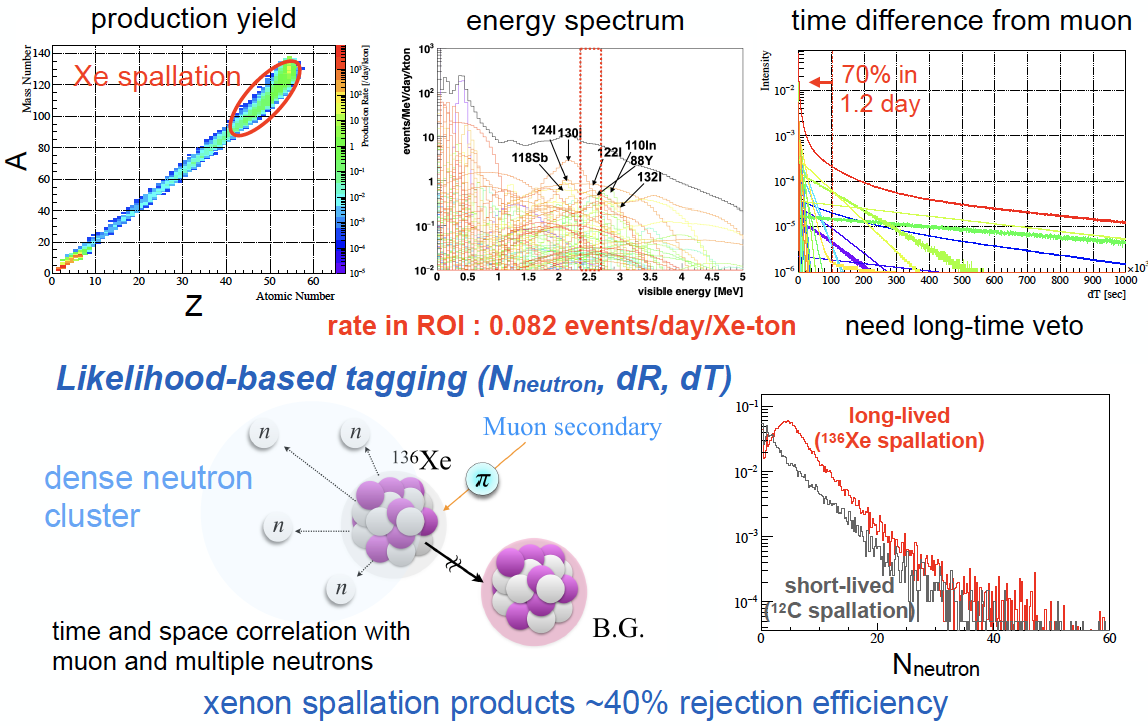
\includegraphics[scale=0.30]{spalallation.png}
\end{frame}

\begin{frame}{Long-lived spallation products}
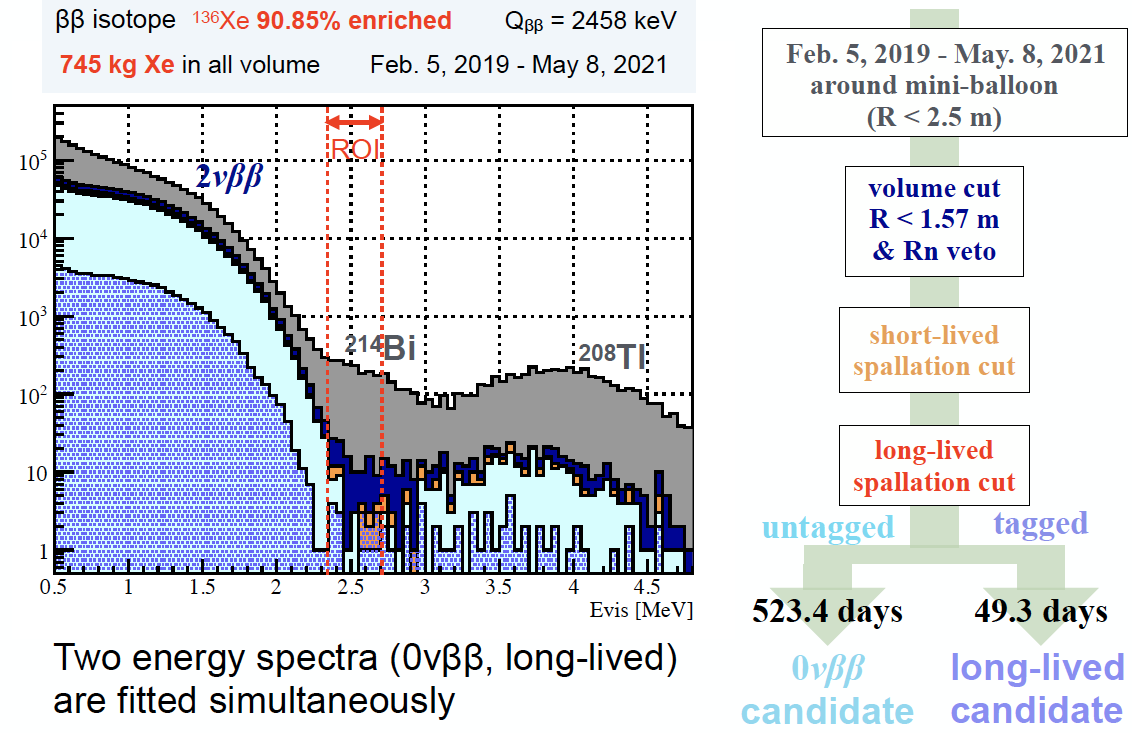
\includegraphics[scale=0.30]{kzeventselection.png}
\end{frame}

\begin{frame}{Fit to energy spectra}
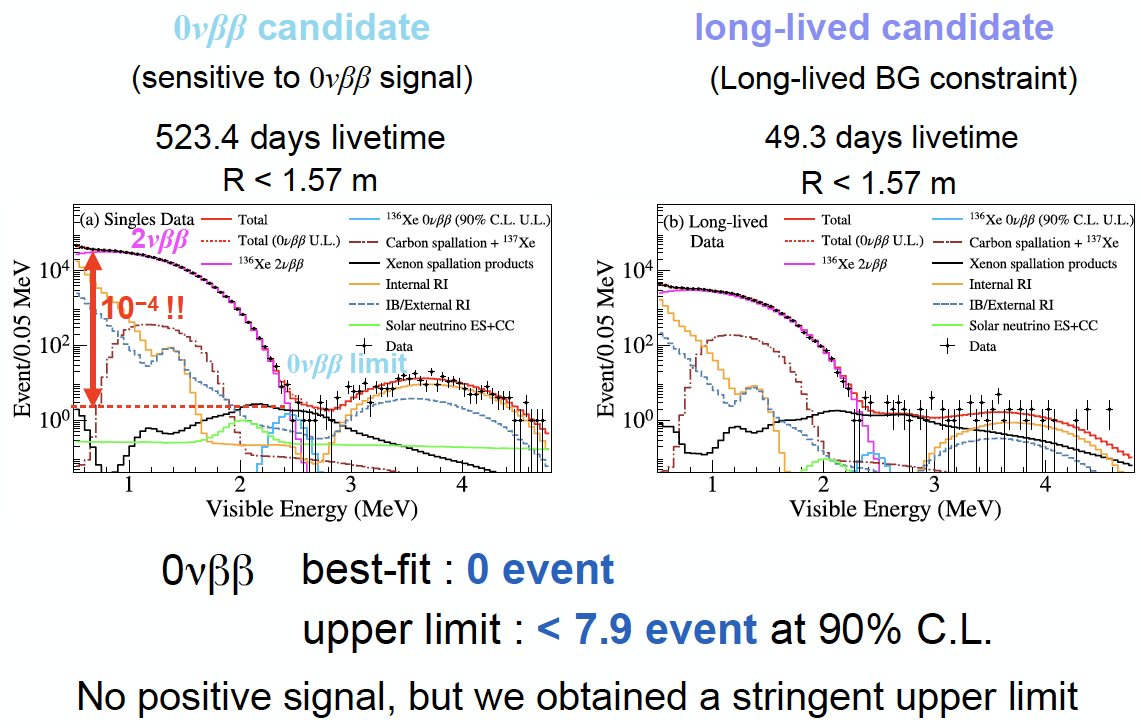
\includegraphics[scale=0.30]{fitkz.png}
\end{frame}

\begin{frame}{Irreducible backgrounds}
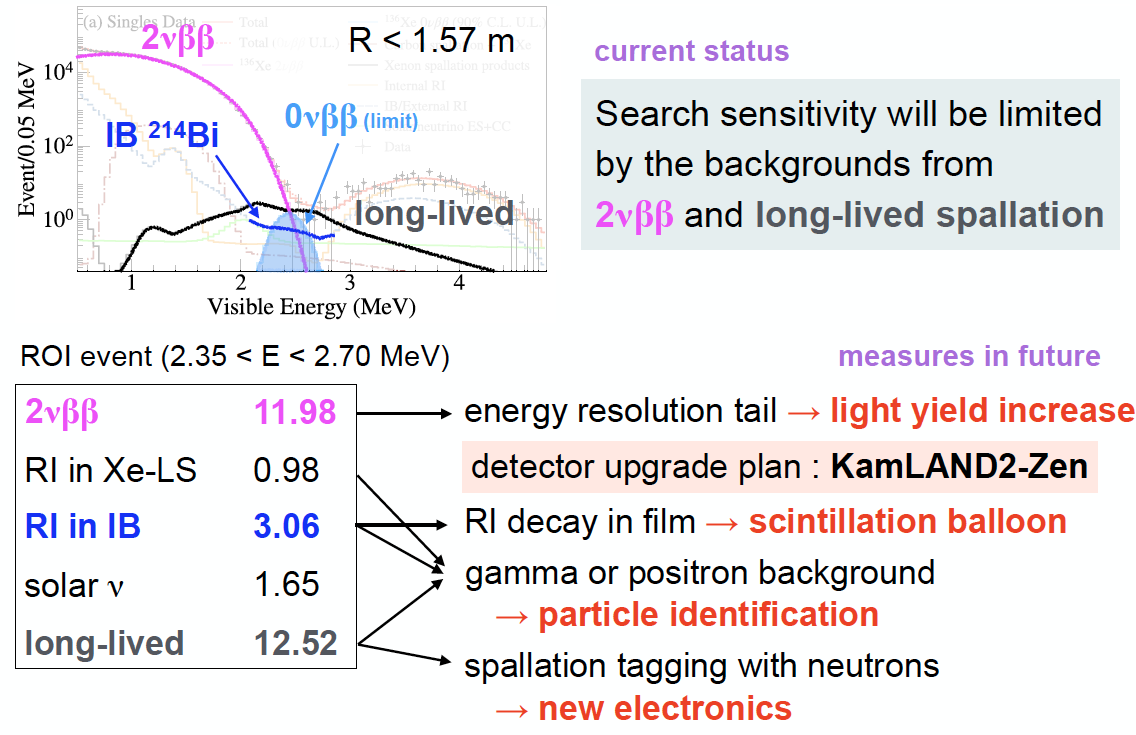
\includegraphics[scale=0.30]{kzsensi.png}
\end{frame}



%%%
\end{document}